\section{Inverse Functions}\label{sec:inv_funcs}

We say that two functions $f$ and $g$ are \emph{inverses} if $g(f(x))=x$ for all $x$ in the domain of $f$ and $f(g(x))=x$ for all $x$ in the domain of $g$. A function can only have an inverse if it is one-to-one, i.e. if we never have $f(x_1)=f(x_2)$ for different elements $x_1$ and $x_2$ of the domain. This is equivalent to saying that the graph of the function passes the horizontal line test.
%Functions that are not one-to-one may sometimes have inverses on part of their domains.
%
%If $f$ and $g$ are inverses, the domain of $g$ will be the range of $f$ and the range of $g$ will be the domain of $f$. The graphs of $f$ and $g$ will be reflections of each other across the line $y=x$ since $y=f(x)$ if and only if $x=g(y)$ (since the point $(y,x)$ is on the graph of $g$ whenever $(x,y)$ is on the graph of $f$.)
The inverse of $f$ is denoted $f^{-1}$, which should not be confused with the function $1/f(x)$.\index{one-to-one}

\begin{keyidea}[Inverse Functions]\label{ki_inv_funcs}
For a one-to–one function $f$,
\begin{itemize}
\item The domain of $f^{-1}$ is the range of $f$; the range of $f^{-1}$ is the domain of $f$.
\item $f^{-1}(f(x))=x$ for all $x$ in the domain of $f$.
\item $f(f^{-1}(x))=x$ for all $x$ in the domain of $f^{-1}$.
\item The graph of $y=f^{-1}(x)$ is the reflection across $y=x$ of the graph of $y=f(x)$.
\item $y=f^{-1}(x)$ if and only if $f(y)=x$ and $y$ is in the domain of $f$.
\end{itemize}
\end{keyidea}

\youtubeVideo{BmjbDINGZGg}{Finding the Inverse of a Function or Showing One Does not Exist, Ex 3}

To determine whether or not $f$ and $g$ are inverses for each other, we check to see whether or not $g(f(x))=x$ for all $x$ in the domain of $f$,and $f(g(x))=x$ for all $x$ in the domain of $g$.

\mtable[-2\baselineskip]{A function $f$ along with its inverse $f\primeskip^{-1}$. (Note how it does not matter which function we refer to as $f$; the other is $f\primeskip^{-1}$.)}{fig_inverse1}{\begin{tikzpicture}
 \begin{axis}[width=1.16\marginparwidth,axis equal,tick label style={font=\scriptsize},
   minor x tick num=1,minor y tick num=1,axis y line=middle,axis x line=middle,
   ymin=-1.2,ymax=1.7,xmin=-1.2,xmax=1.7,name=myplot]
  \addplot[draw={\colorone},smooth,thick,domain=-1:1.05] (x,x^3+.5);
  \addplot[draw={\colortwo},smooth,thick,domain=-1:1.05] (x^3+.5,x);
  \addplot[dashed,thin] {x};
  \filldraw[black] (axis cs:-.5,.375)
   node [shift={(-10pt,10pt)}] {\tiny $(-0.5,0.375)$} circle (1pt);
  \filldraw[black] (axis cs:.375,-.5)
   node [shift={(10pt,-10pt)}] {\tiny $(0.375,-0.5)$} circle (1pt);
  \filldraw[black] (axis cs:1,1.5) node [left] {\tiny $(1,1.5)$} circle (1pt);
  \filldraw[black] (axis cs:1.5,1) node [below] {\tiny $(1.5,1)$} circle (1pt);
 \end{axis}
 \node[right] at (myplot.right of origin) {\scriptsize $x$};
 \node[above] at (myplot.above origin) {\scriptsize $y$};
\end{tikzpicture}}

\begin{example}[Verifying Inverses]\label{ex_inv_determine}
Determine whether or not the following pairs of functions are inverses:
\begin{enumerate}
\item $f(x)=3x+1$; $g(x)=\dfrac{x-1}3$
\item $f(x)=x^3+1$; $g(x)=x^{1/3}-1$
\end{enumerate}
\solution
\begin{enumerate}
\item To check the composition we plug $f(x)$ in for $x$ in the definition of $g$ as follows:\vspace{-.3\baselineskip}
\[ g(f(x))=\frac{f(x)-1}3=\frac{(3x+1)-1}3=\frac{3x}3=x\]
So $g(f(x))=x$ for all $x$ in the domain of $f$. Likewise, you can check that $f(g(x))=x$ for all $x$ in the domain of $g$, so $f$ and $g$ are inverses.
\item If we try to proceed as before, we find that:
\[g(f(x))=(f(x))^{1/3}-1=(x^3+1)^{1/3}-1\]
This doesn't seem to be the same as the identity function $x$. To verify this, we find a number $a$ in the domain of $f$ and show that $g(f(a))\neq a$ for that value. Let's try $x=1$. Since $f(1)=1^3+1=2$, we find that $g(f(1))=g(2)=2^{1/3}-1\approx 0.26$. Since $g(f(1))\neq 1$, these functions are not inverses.
\end{enumerate}
\end{example}

%To find the inverse $f^{-1}$ of a given function $y=f(x)$, we follow these steps (when possible):
%\begin{enumerate}
%\item In the equation defining $f$, solve for $x$.
%\item Interchange $x$ and $y$.
%\item The equation now defines $y=f^{-1}(x)$.
%\end{enumerate}
%
%\begin{example}[Finding Inverses]\label{ex_inv_find}
%Find the inverses of the following functions.
%\[\text{1.}\quad f(x)=5x+3\qquad\qquad\text{2.}\quad g(x)=x^3+1.\]
%\solution\begin{enumerate}
%\item Start with the equation $y=5x+3$ and solve for $x$:
%\begin{align*}
%y&=5x+3\\
%y-3&=5x\\
%\frac{y-3}5 &=x
%\end{align*}
%Next interchange $x$ and $y$ to get $y=\dfrac{x-3}5$. The inverse of $f$ is:
%\[ f^{-1}(x)=\frac{x-3}5 \]
%\item Proceeding as before, we get:
%\begin{align*}
%y&=x^3+1\\
%y-1&=x^3\\
%(y-1)^{1/3}&=x
%\end{align*}
%Interchanging $x$ and $y$ yields $y=(x-1)^{1/3}$, so
%\[g^{-1}(x)=(x-1)^{1/3}.\]
%\end{enumerate}
%\end{example}


\subsection{Functions that are not one-to-one.}

\mtable{The function $f(x)=x^2$ is not one-to-one.}{fig_parab_oto}{\begin{tikzpicture}
 \begin{axis}[width=\marginparwidth,
   tick label style={font=\scriptsize},axis y line=middle,axis x line=middle,
   ymin=-1,ymax=5,xmin=-2.5,xmax=2.5,xtick={-2,2},ytick={},name=myplot]
  \addplot [draw={\colorone},smooth,thick,domain=-2.5:2.5] (x,{x^2});
  \draw (axis cs:-2,4)node[above right]{\scriptsize$(-2,4)$}
      --(axis cs:2,4)node[above left]{\scriptsize$(2,4)$};
 \end{axis}
 \node [right] at (myplot.right of origin) {\scriptsize $x$};
 \node [above] at (myplot.above origin) {\scriptsize $y$};
\end{tikzpicture}}
Unfortunately, not every function we would like to find an inverse for is one-to-one. For example, the function $f(x)=x^2$ is not one-to-one because $f(-2)=f(2)=4$. If $f^{-1}$ is an inverse for $f$, then $f^{-1}(f(-2))=-2$ implies that $f^{-1}(4)=-2$. On the other hand, $f^{-1}(f(2))=2$, so $f^{-1}(4)=2$. We cannot have it both ways if $f^{-1}$ is a function, so no such inverse exists. We can find a partial solution to this dilemma by restricting the domain of $f$. There are many possible choices, but traditionally we restrict the domain to the interval $[0,\infty)$. The function $f^{-1}(x)=\sqrt x$ is now an inverse for this restricted version of $f$.


\subsection{The inverse sine function}

We consider the function $f(x)=\sin x$, which is not one-to-one. A piece of the graph of $f$ is in \autoref{fig_sin_arc}(a). In order to find an appropriate restriction of the domain of $f$, we look for consecutive critical points where $f$ takes on its minimum and maximum values. In this case, we use the interval $[-\pi/2,\pi/2]$. We define the inverse of $f$ on this restricted range by $y=\sin^{-1}x$ if and only if $\sin y=x$ and $-\pi/2\leq y\leq \pi/2$. The graph is a reflection of the graph of $g$ across the line $y=x$, as seen in \autoref{fig_sin_arc}(b).

\noindent\begin{minipage}[t]{\linewidth}\noindent%
\captionsetup{type=figure}%
\centering
\tagpdfsetup{table/header-rows={2}}
\begin{tabular}{cc}
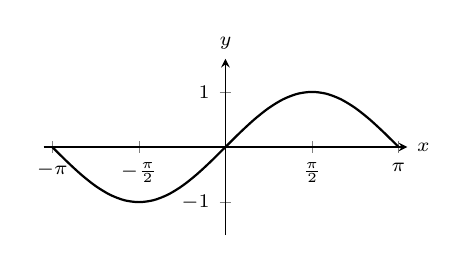
\begin{tikzpicture}[baseline={(current bounding box.center)}]
 \begin{axis}[x=.7cm, y=.7cm,
   tick label style={font=\scriptsize},axis y line=middle,axis x line=middle,
   ymin=-1.6,ymax=1.6,xmin=-3.3,xmax=3.3,xtick={-3.14,-1.57,1.57,3.14},
   xticklabels={$-\pi$,$-\frac\pi2$,$\frac\pi2$,$\pi$},name=myplot]
  \addplot [draw={\colorone},smooth,thick,domain=-3.14:3.14] (x,{sin(deg(x))});
 \end{axis}
 \node[anchor=base] at (myplot.origin) {};
 \node [right] at (myplot.right of origin) {\scriptsize $x$};
 \node [above] at (myplot.above origin) {\scriptsize $y$};
\end{tikzpicture}
&
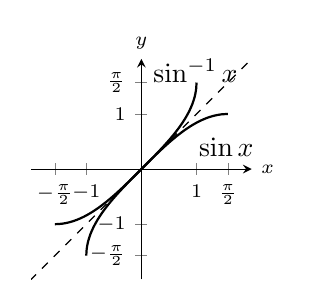
\begin{tikzpicture}[baseline={(current bounding box.center)}]
 \begin{axis}[x=.7cm,y=.7cm,
   tick label style={font=\scriptsize},axis y line=middle,axis x line=middle,
   ymin=-2,ymax=2,xmin=-2,xmax=2,name=myplot,
   xtick={-1.57,-1,1,1.57},xticklabels={$-\frac\pi2$,$-1$,$1$,$\frac\pi2$},
   ytick={-1.57,-1,1,1.57},yticklabels={$-\frac\pi2$,$-1$,$1$,$\frac\pi2$}]
  \addplot [draw={\colorone},smooth,thick,domain=-1.57:1.57] (x,{sin(deg(x))})
   node[pos=.8,below right]{$\sin x$};
  \addplot [draw={\colortwo},smooth,thick,domain=-1.57:1.57] ({sin(deg(x))},x)
   node[pos=.95,above]{$\sin^{-1}x$};
  \addplot[dashed,thin] {x};
 \end{axis}
 \node[anchor=base] at (myplot.origin) {};
 \node [right] at (myplot.right of origin) {\scriptsize $x$};
 \node [above] at (myplot.above origin) {\scriptsize $y$};
\end{tikzpicture}
\\ (a) & (b)
\end{tabular}
\caption{(a) A portion of $y=\sin x$. (b) A one-to-one portion of $y=\sin x$ along with $y=\sin^{-1}x$.}
\label{fig_sin_arc}
\end{minipage}

\subsection{The inverse tangent function}

Next we consider the function $f(x)=\tan x$, which is also not one-to-one. A piece of the graph of $f$ is given in \autoref{fig_tan_arc}(a).  In order to find an interval on which the function is one-to-one and on which the function takes on all values in the range, we use an interval between consecutive vertical asymptotes. Traditionally, the interval $(-\pi/2,\pi/2)$ is chosen. Note that we choose the open interval in this case because the function $f$ is not defined at the endpoints. So we define $y=\tan^{-1} x$ if and only if $\tan y=x$ and $-\pi/2< y<\pi/2$. The graph of $y=\tan^{-1} x$ is shown in \autoref{fig_tan_arc}(b). Also note that the vertical asymptotes of the original function are reflected to become horizontal asymptotes of the inverse function.

\noindent\begin{minipage}[t]{\linewidth}\noindent%
\captionsetup{type=figure}%
\centering
\tagpdfsetup{table/header-rows={2}}
\begin{tabular}{cc}
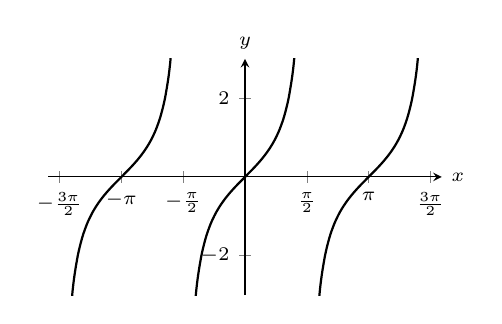
\begin{tikzpicture}[baseline={(current bounding box.center)}]
 \begin{axis}[x=.5cm,y=.5cm,
   tick label style={font=\scriptsize},axis y line=middle,axis x line=middle,
   ymin=-3,ymax=3,xmin=-5,xmax=5,xtick={-4.71,-3.14,-1.57,1.57,3.14,4.71},
   xticklabels={$-\frac{3\pi}2$,$-\pi$,$-\frac\pi2$,$\frac\pi2$,$\pi$,$\frac{3\pi}2$},
   name=myplot]
  \addplot [draw={\colorone},smooth,thick,domain=-1.5:1.5] (x,{tan(deg(x))});
  \addplot [draw={\colorone},smooth,thick,domain=-1.5:1.5] (x+3.14,{tan(deg(x))});
  \addplot [draw={\colorone},smooth,thick,domain=-1.5:1.5] (x-3.14,{tan(deg(x))});
 \end{axis}
 \node [right] at (myplot.right of origin) {\scriptsize $x$};
 \node [above] at (myplot.above origin) {\scriptsize $y$};
\end{tikzpicture}
&
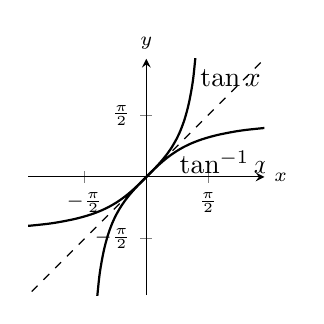
\begin{tikzpicture}[baseline={(current bounding box.center)}]
 \begin{axis}[x=.5cm,y=.5cm,
   tick label style={font=\scriptsize},axis y line=middle,axis x line=middle,
   ymin=-3,ymax=3,xmin=-3,xmax=3,name=myplot,
   xtick={-1.57,1.57},xticklabels={$-\frac\pi2$,$\frac\pi2$},
   ytick={-1.57,1.57},yticklabels={$-\frac\pi2$,$\frac\pi2$}]
  \addplot [draw={\colorone},smooth,thick,domain=-1.3:1.3] (x,{tan(deg(x))})
   node[pos=.8,above right]{$\tan x$};
  \addplot [draw={\colortwo},smooth,thick,domain=-1.3:1.3] ({tan(deg(x))},x)
   node[pos=.6,below right,yshift=1.3ex]{$\tan^{-1}x$};
  \addplot[dashed,thin] {x};
 \end{axis}
 \node [right] at (myplot.right of origin) {\scriptsize $x$};
 \node [above] at (myplot.above origin) {\scriptsize $y$};
\end{tikzpicture}
\\ (a) & (b)
\end{tabular}
\caption{(a) A portion of $y=\tan x$. (b) A one-to-one portion of $y=\tan x$ along with $y=\tan^{-1}$.}
\label{fig_tan_arc}
\end{minipage}

The other inverse trigonometric functions are defined in a similar fashion. The resulting domains and ranges are summarized in \autoref{fig:domain_trig}.\bigskip

\noindent\begin{minipage}[t]{\linewidth}\noindent%
\captionsetup{type=figure}%
\small%
\flushinner{%
\tagpdfsetup{table/header-rows={1}}
\begin{tabular}{ c c c @{\hspace{2em}} c c c }
Function & \parbox[b]{40pt}{\centering Restricted Domain} & Range &\parbox[b]{40pt}{\centering Inverse Function} & Domain & Range\\ \cmidrule(r{2em}){1-3}\cmidrule(l{-1em}){4-6}
$\sin x$ & $[-\pi/2,\pi/2]$ & $[-1,1]$&$\sin^{-1}x$ & $[-1,1]$ & $[-\pi/2,\pi/2]$ \\
$\cos x$ & $[0,\pi]$ & $[-1,1]$&$\cos^{-1}x$ & $[-1,1]$ & $[0,\pi]$ \\
$\tan x$ & $(-\pi/2,\pi/2)$ & $(-\infty,\infty)$ & $\tan^{-1}x$ & $(-\infty,\infty)$ & $(-\pi/2,\pi/2)$	\\
$\csc x$ & $[-\pi/2,0)\cup (0, \pi/2]$ & $(-\infty,-1]\cup [1,\infty)$&$\csc^{-1} x$ & $(-\infty,-1]\cup [1,\infty)$ & $[-\pi/2,0)\cup (0, \pi/2]$  \\
$\sec x$ & $[0,\pi/2)\cup (\pi/2,\pi]$ & $(-\infty,-1]\cup [1,\infty)$&$\sec^{-1}x$ & $(-\infty,-1]\cup [1,\infty)$ & $[0,\pi/2)\cup (\pi/2,\pi]$ \\
$\cot x$ & $(0,\pi)$ & $(-\infty,\infty)$&$\cot^{-1}x$ &  $ (-\infty,\infty)$ & $(0,\pi)$	
\end{tabular}}
\caption{Domains and ranges of the trigonometric and inverse trigonometric functions.}
\label{fig:domain_trig}
\end{minipage}

\begin{example}[Evaluating Inverse Trigonometric Functions]\label{eg_inv_trig}
Find exact values for the following:
\mnote[-\baselineskip]{Sometimes, $\arcsin$ is used instead of $\sin^{-1}$.  Similar ``arc'' functions are used for the other inverse trigonometric functions as well.}
\\
\begin{minipage}{.5\linewidth}
\begin{enumerate}
 \item $\tan^{-1}(1)$
 \item $\cos(\sin^{-1}(\sqrt3/2))$
\end{enumerate}
\end{minipage}%
\begin{minipage}{.5\linewidth}
\begin{enumerate}
 \setcounter{enumi}{2}
 \item $\sin^{-1}(\sin(7\pi/6))$
 \item $\tan(\cos^{-1}(11/15))$
\end{enumerate}
\end{minipage}
\solution
\begin{enumerate}
\item $\tan^{-1}(1)=\pi/4$
\item $\cos(\sin^{-1}(\sqrt3/2))=\cos(\pi/3)=1/2$
\item Since $7\pi/6$ is not in the range of the inverse sine function, we should be careful with this one.
\[\sin^{-1}(\sin(7\pi/6))=\sin^{-1}(-1/2)=-\pi/6.\]
\item Since we don't know the value of $\cos^{-1}(11/15)$, we let $\theta$ stand for this value. We know that $\theta$ is an angle between $0$ and $\pi$ and that $\cos(\theta)=11/15$.
In \autoref{fig_inv_trig}, we use this information to construct a right triangle with angle $\theta$, where the adjacent side over the hypotenuse must equal 11/15. Applying the Pythagorean Theorem we find that
\mtable[-\baselineskip]{A right triangle for the situation in \autoref{eg_inv_trig} (4).}{fig_inv_trig}{%
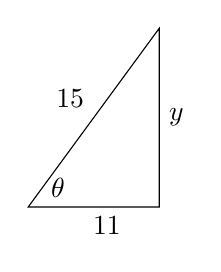
\begin{tikzpicture}[x=1ex,y=1ex]
 \draw(0,0)
  --node[pos=.1,above right]{$\theta$}node[pos=.6,below]{11}(11,0)
  --node[pos=.5,right]{$y$}(11,15)
  --node[pos=.5,above left]{15}cycle;
\end{tikzpicture}}
\[y=\sqrt{15^2-11^2}=\sqrt{104}=2\sqrt{26}.\]
Finally, we have:
\[\tan(\cos^{-1}(11/15))=\tan(\theta)=\frac{2\sqrt{26}}{11}.\]
\end{enumerate}
\end{example}

\printexercises{exercises/07-07-exercises}

% todo write an example of finding the inverse of a function

% todo write more exercises for 7.1
